\documentclass{book}

\usepackage{hyperref}
\usepackage{graphicx}
\usepackage[letterpaper, margin=1in]{geometry}
\usepackage{amsmath}
\usepackage{amsfonts}
\usepackage{cleveref}
\newtheorem{definition}{Definition}
\newtheorem{theorem}{Theorem}


\graphicspath{{./fig/}}

\title{Lie Groups in Robotics}
\author{James Goppert}
\date{January 22, 2023}

\begin{document}

\maketitle
\tableofcontents

\chapter{Introduction}

This book is aimed at introducing graduate and undergraduate students
in engineering to the applications of Lie groups theory that are 
relevant to engineering. Instead of focusing on the abstract 
mathematics initially, it will build intuition by traversing the most
fundamental Lie Groups in robotics.

\section{What is a Lie Group}

\begin{definition}
A \href{https://en.wikipedia.org/wiki/Group_(mathematics)}{Group} is a set G
and an associated operator $\cdot$ that is:
\begin{itemize}
    \item \textbf{C}losed: if $a \in G$ and $b \in G$, then $a \cdot b \in G$
	\item \textbf{A}ssociative: $(a \cdot b) \cdot c = a \cdot (b \cdot c)$
    \item \textbf{I}nverse: $a^{-1}\cdot a = e$
    \item \textbf{N}eutral: $a \cdot e = a$
\end{itemize}
\end{definition}

\begin{definition}
    A \href{https://en.wikipedia.org/wiki/Lie_group}{Lie Group} is a group that
    is also a differentiable manifold.
    \end{definition}

A \href{https://en.wikipedia.org/wiki/Differentiable_manifold}{differentiable manifold}
is a topological space resemlbling Euclidean space near each point
and locally similar enough to a vector space to apply calculus. Originally Lie Groups were called infinitesmal groups by the creator
\href{https://en.wikipedia.org/wiki/Sophus_Lie}{Sophus Lie} (pronounced Lee).
The can be thought of as groups of continuous transformations.

\begin{figure}[htp]
    \centering
    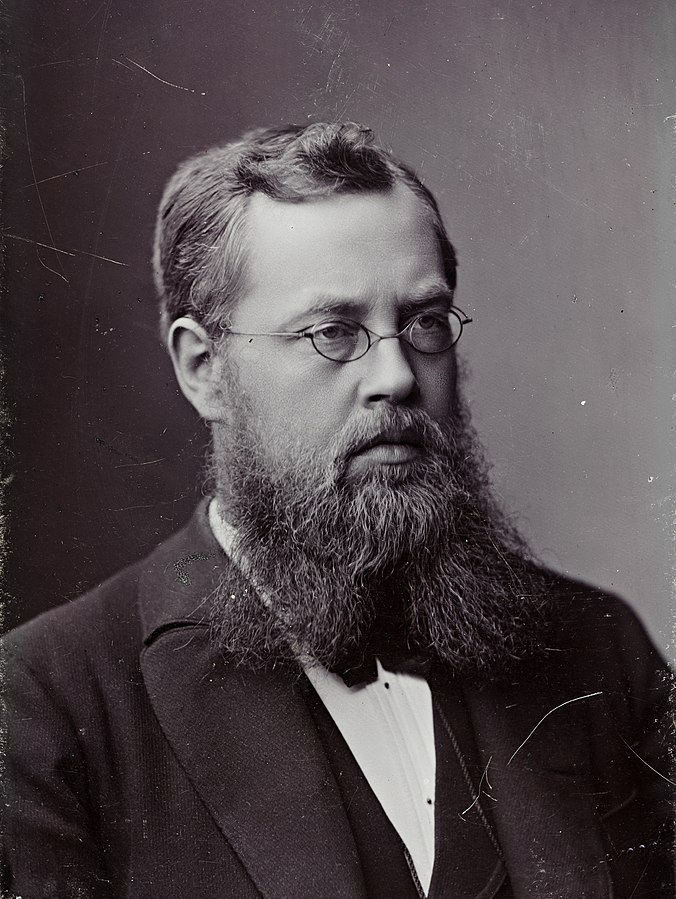
\includegraphics[width=100px]{sophus_lie}
    \caption{Sophus Lie}
\end{figure}

\section{Applications of Lie Groups}

\subsection*{Covered in this Course}
\begin{itemize}
    \item Estimation
        \begin{itemize}
            \item IEKF : Invariant Extended Kalman Filter
            \item Simultaneous Localization and Mapping
        \end{itemize}
    \item Control of Rigid Bodies
        \begin{itemize}
            \item Reachable set calculations
            \item Geometric control
        \end{itemize}
    \item Computer Vision
    \begin{itemize}
        \item Perspective Transforms
        \item Homogenous Coordinates
    \end{itemize}
\end{itemize}


\subsection*{Others Topics not Covered}
\begin{itemize}
    \item Quantum mechanics
\end{itemize}


\section*{Excercises}

\subsection*{Questions about Groups}

\begin{itemize}
    \item Is the set of all Integers $\mathbb{Z}$ with the addition operator $+$ a group?
    \item Is the set of all Integers $\mathbb{Z}$ with the multiplication operator $*$ a group?
    \item Is the set of all $n\times n$ matrices with the matrix multiplication oerator a group?
\end{itemize}

\subsection*{Questions about Lie Groups}
\begin{itemize}
    \item Is the set of all Integers $\mathbb{Z}$ with the addition operator $+$ a Lie group?
    \item Is the set of all Real numbers $\mathbb{R}$ with the addition operator $+$ a Lie group?
\end{itemize}


\chapter{The SO(2) Lie Group}
%
\section{Group Representation}
%
$SO(2)$ can be represented by any matrix of the from:
%
$$G(\theta) = \begin{bmatrix}
\cos{\theta} & -\sin{\theta} \\
\sin{\theta} & \cos{\theta}
\end{bmatrix}$$
with the Group operator of matrix multiplication ($\cdot$), where $\theta \in \mathbb{R}$.

To show that $SO(2)$ is a Lie Group, we much show that it is closed, associative, has inverse, and a neutral element and is a differentiable manifold

\subsection*{Closed}
%
Since $G(\theta_1) \cdot G(\theta_2) = G(\theta_1 + \theta_2)$, $SO(2)$ is \textbf{closed} under matrix multiplication.

\subsection*{Associative}
%
$SO(2)$ as a Matrix Lie Group, can inheret associativity from matrix multiplication:
%
$$(A \cdot B) \cdot C = A \cdot (B \cdot C)$$

\subsection*{Inverse}
%
$SO(2)$ as a Matrix Lie Group, can inheret the inverse from matrix multiplication, since any element of $SO(2)$ has a non-zero determinant (1) and is invertible.
%
$$\det{G} = \cos^2{\theta} + \sin^2{\theta} = 1$$
%
Because the columns of $G(\theta)$ are orthonomal, the inverse is given by the matrix transpose.
%
$$G^{-1}(\theta) = G^T(\theta)$$

\subsection*{Neutal}
%
$SO(2)$ as a Matrix Lie Group, can inheret the neutral element from matrix multiplication, $I$.
%
$$A\cdot I = A$$

\subsection*{Differential Manifold}
Is is clear that the group $SO(2)$ is continuous as it inherits this from $\mathbb{R}$.
$G(\theta)$, $\theta \in \mathbb{R}$.
We will see in the Lie Algebra that the group is locally similar to 1 dimensional Euclidean space
and we can perform calculus.


\section{Lie Algebra}
%
An algebra is a set with associated operators for addition/subtraction, multiplication/division.
$\mathcal{R}^3$, the space of 3-dimensions vectors forms an algebra. We are familiar with the cross product and vector addition.
Vector addition acts as the addition/subtraction operator and the cross product acts as the multiplication/division operator.

The associated Lie algebra of a Lie group is a linear vector space and already is closed under the addition and subtract operator.
The Lie bracket \cref{def:lie_bracket}, which we will study soon, acts as the multiplication/division operator.
%
For matrix Lie groups, we can always find an element of the Lie Algebra, $\Omega$ via:
%
$$\dot{G} = G\Omega$$
%
$$\Omega = G^{-1}\dot{G}$$
%
The so2 Lie algebra can be represented by all 2x2 skew symmetric matrices of the form:
%
$$\Omega = \begin{bmatrix}
0 & - \omega\\
\omega & 0
\end{bmatrix}$$
%
It is convenient to define a wedge operator such that:

\begin{definition}[The Wedge Operator]
$$\mathbb{R} \mapsto so(2)$$
$$\omega^{\wedge} = \begin{bmatrix}
    0 & - \omega\\
    \omega & 0
    \end{bmatrix}$$
\end{definition}
%
It is also convient to define a vee operator, the inverse of the wedge operator such that:
%
\begin{definition}[The Vee Operator]
$$so(2) \mapsto \mathbb{R}$$
$$\begin{bmatrix}
0 & - \omega\\
\omega & 0
\end{bmatrix}^{\vee} = \omega$$
\end{definition}

\section{The Exponential Map}

\begin{definition}[The Lie Group Exponential Map]
The Lie group Exponential map maps from the Lie algebra to the Lie group.
For matrix Lie groups, such as $SO(2)$ it is given by the matrix
exponential.
\end{definition}

\begin{definition}[The Lie Group Logarithm Map]
The Lie group logarithm map maps from the Lie group to the Lie algebra.
For matrix Lie groups, such as $SO(2)$ it is given by the matrix
logarithm, the inverse of the matrix exponential.
\end{definition}

\begin{figure}[htp]
    \centering
    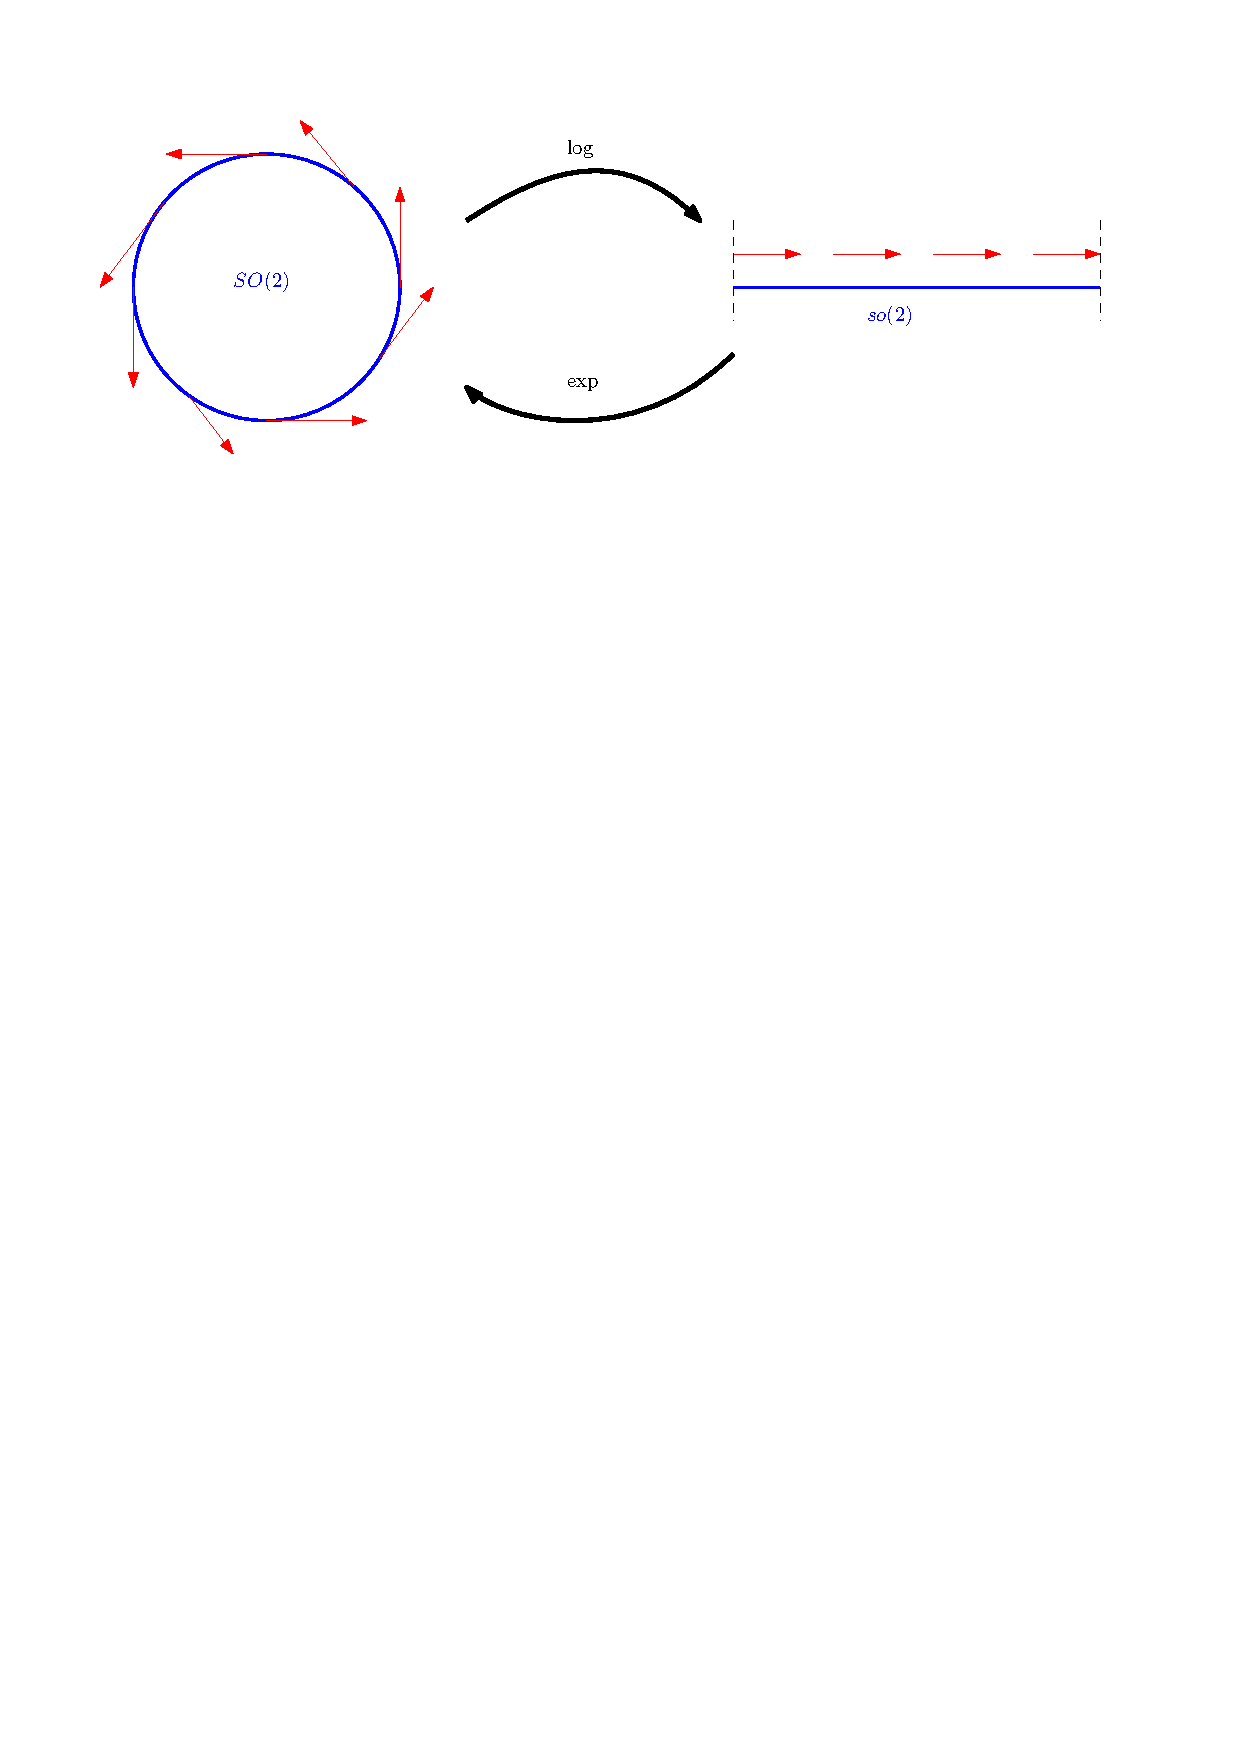
\includegraphics[width=\textwidth]{SO2_so2_vector_field}
    \caption{Transformation of a Vector Field from the Lie Group to the Lie Algebra}
\end{figure}

\begin{definition}[Bijective/Invertible Map]
A map is bijective or invertible if it is:
\begin{itemize}
    \item One-one/ injective: For each point in the domain there is one point in the range.
    \item Onto/ surjective: Each point in the range is mapped to by a point in the domain.
\end{itemize}
\end{definition}

It is often beneficial for us to map vector fields to the Lie algebra to simplify
analysis. If we do this, we desire an invertible map, so after we take the logarithm,
we can then take the exponential of the Lie algebra to obtain results in the Lie group.
We will see later how this can be used for reachable set computation. It is important
to note that the matrix exponential is not one to one. A single point in the range, can be
reached by multiple points in the domain, since for $so(2)$, the Lie algebra parameter $\theta$ 
and $\theta + 2\pi k$, $k\in \mathbb{Z}$, map to the same point. However, we can restrict the
comain of the map to $\{-\pi, \pi\}$ and the map is invertible in this domain.

\section{Vector Fields}

On a Lie group, a vector field can be represented by an element of the Lie algebra. This element
can then be pushed forward to other group elements, and defining the derivative of the Lie group
element at that point.

There are two types of vector fields that may be defined.

\begin{definition}[Left Invariant Vector Fields]
A vector field is left invariant, if multiplying on the left by an element of the
group does not modify the vector field. Define a group element $G_t$ as the product of a constant group element $A$, and a time
varying group element $B_t$, $G_t = A B_t$. Here we use the notation that
 $A_t$ indicates that $A$ is a function of time. Then:

$$\dot{B_t} = B_t [\omega]^{\wedge} \implies \dot{G_t} = G_t [\omega]^{\wedge} $$

$$\dot{G_t} = \dfrac{d}{dt} \left(A B_t \right) = A B_t [\omega]^{\wedge} = G_t [\omega]^{\wedge} $$
\end{definition}

\begin{definition}[Right Invariant Vector Fields]
A vector field is right invariant, if multiplying on the right by an element of the
group does not modify the vector field. Define a group element $G_t$ as the product of a time
varying group element $A_t$, and a constant group element $B$, $G_t = A_t B$.

$$\dot{A_t} = [\omega]^{\wedge} A_t  \implies \dot{G_t} = [\omega]^{\wedge} G_t$$

$$\dot{G_t} = \dfrac{d}{dt} \left(A_t B \right) = [\omega]^{\wedge}  A_t B = [\omega]^{\wedge} G_t$$
\end{definition}

\begin{definition}[Combing a Vector Field]
A vector field may be combed by a Lie algebra element, if one Lie algebra element can 
define a vector field on the group without a singularity.
\end{definition}

\section{The Lie bracket and Adjoint operators, Ad and ad}

The Adjoint map maps element from the Lie algebra from one tangent space to another.

$$\dot{G_t} = G_t [\omega_l]^{\wedge} = [\omega_r]^{\wedge} G_t $$

$$\dot{G_t}  G_t^{-1}  = G_t [\omega_l]^{\wedge} G_t^{-1} = [\omega_r]^{\wedge}$$

$$[\omega_r]^{\wedge} = G_t [\omega_l]^{\wedge} G_t^{-1}$$


\begin{definition}[$Ad$ operator]
The Adjoint operator maps a Lie algebra element $[\omega]^{\wedge}$
at the origin(e), to the tangent at $G_t$ is given by:
$$g \mapsto g$$ where g is an element of the Lie algebra
$$Ad_{G_t}[\omega]^{\wedge} \equiv G_t [\omega]^{\wedge} G_t^{-1}$$
\label{def:Ad}
\end{definition}
%
\begin{theorem} [Linearity of $Ad_G$ operator]
$Ad_G$ is a linear operator on the Lie algebra for any Lie Group (it can be represented as a matrix)
when the components of $\omega$ are expressed as a vector in $\mathcal{R}^n$, where n is the dimension
of the Lie algebra.
$$\mathcal{R}^n \mapsto \mathcal{R}^n$$ where n is the dimension of the Lie alegbra.
$$Ad_G \omega_1 = \omega_2$$
\label{thm:lin_Ad}
\end{theorem}
%
The use of the linear operator (matrix) form of Ad, as defined in \cref{thm:lin_Ad} will
be implied when multiplying a vector (e.g.  $(\omega_2 = Ad_{G_t} \omega_1$). The use of the
operator as defined in \cref{def:Ad} in will be implied when multiplying by an element of the Lie algebra,
(e.g. $Ad_{G_t}\left([\omega]^{\wedge}\right)$)

%TODO, show proof
The $ad$ operator is derived by taking the derivative of the $Ad$ operator at the origin.
%
\begin{definition}[$ad_x y$ operator]
$$ad_{[\omega_1]^{\wedge}} [\omega_2]^{\wedge} \equiv [\omega_1]^{\wedge} [\omega_2]^{\wedge} - [\omega_2]^{\wedge} [\omega_1]^{\wedge}$$
\end{definition}
%
\begin{definition}[Lie bracket operator]
The Lie bracket is a binary operator, denoted by $\left[ \cdot , \cdot \right]$,  that acts as the multiplication operator for Lie algebras. It is equivalent to the ad operator.
$$\left[[\omega_1]^{\wedge}, [\omega_2]^{\wedge}\right] \equiv ad_{[\omega_1]^{\wedge}} [\omega_2]^{\wedge} \equiv [\omega_1]^{\wedge} [\omega_2]^{\wedge} - [\omega_2]^{\wedge} [\omega_1]^{\wedge}$$
\label{def:lie_bracket}
\end{definition}
%

\section*{Exercises}

\begin{enumerate}
    \item Prove that $SO2$ is a group.
    \item By hand, take the matrix exponential of the Lie algebra of $se(2)$ and show that it
      maps to the Lie group $SO2$.
    \item Which vector fields of $so(2)$ can comb $SO(2)$? Is there a vector-field as a
      function of $\theta$, defined in $so(2)$ that does not comb $SO(2)$.
    \item Write a class in python that represents the group $SO(2)$ and the Lie algebra $so(2)$.
      It should implement the group product, neutral element, inverse, exponential map,
      and the logarithm map. Use this class to programmatically find $log(exp^\wedge(\theta_1)exp^\wedge(\theta_2))$.
      Evaluate this for $\theta_1=1$ and $\theta_2=2$.  Here $G(\theta)$ indicates the group element with parameter $\theta$.
\end{enumerate}

\end{document}
